\documentclass{article}
\usepackage[utf8]{inputenc}
\usepackage{graphicx}
\usepackage{hyperref}
\usepackage{array}
\usepackage{wrapfig}
\usepackage{multirow}
\usepackage{tabu}

\hypersetup{
    colorlinks=true,
    linkcolor=blue,
    filecolor=magenta,      
    urlcolor=cyan,
}

\title{\line(1,0){250}\\{\Huge \bigskip Gesture Documentation}\\\line(1,0){250}}
\author{ \footnotesize by \\[0.2cm] \footnotesize Gary Connelly (G00336837) \\[0.2cm] \footnotesize \& \\[0.2cm] \footnotesize Conor Raftery (G00274094)}
\date{\footnotesize April 2019}

\begin{document}

\maketitle
\bigskip
\bigskip
\bigskip
\bigskip
\bigskip
\bigskip
\bigskip
\bigskip
\bigskip
\bigskip
\bigskip
\bigskip

\includegraphics[width=\textwidth, height=150pt]{img/gmit-logo.jpg}

\tableofcontents

\clearpage
\section{Introduction}
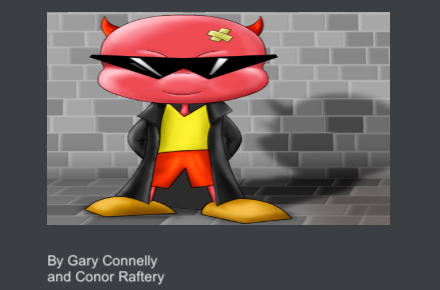
\includegraphics[width=\textwidth, height=180pt]{img/splash2.PNG}

\bigskip


This document looks at the general purpose documentation relating to the project. This project was completed as part of the Gesture Based UI Development module in the 4th year software development course.  This project carries 60\% of the overall grade for this module. This was also a group project. There were two members of the group; Gary Connelly, and Conor Raftery. For this project, the team developed an fully gesture controlled adaption of the original "Bubble Struggle" game. 

\bigskip

The rules of this game are simple, the player can move left and right to avoid the bubbles that are bouncing around the scene. The player can shoot the bubbles using a hook and chain. If they hit a bubble, the bubble will pop into two or more smaller bubbles. This will continue until the bubbles become too small to split, in which case, when they are hit they simply evaporate. The aim of the game is to clear all of the bubbles from the level before the timer runs out and without losing all three lives. A player loses a life if they are hit by a bubble.

\section{Installation Guide}
This project is built using the Unity Engine, specifically version 'Unity 2018.3.12'. This is the recommended version to be installed, although older/newer version may work by upgrading or downgrading the project respectively. 

\bigskip

This project has a pre-built executable file for effortless running of the project. This executable file has been created using the Unity Engine. It can be found within the Github repository within the folder 'Builds'. To access this, download the Github repository, open up the 'Builds' folder, and run the executable file named 'GestureUIProject.exe'. If this fails, or you wish to have a look at the entirety of the project, follow the following steps.

\bigskip

Once Unity has been successfully installed, you must download the project from the Github Repository and import the Assets folder into Unity.\\
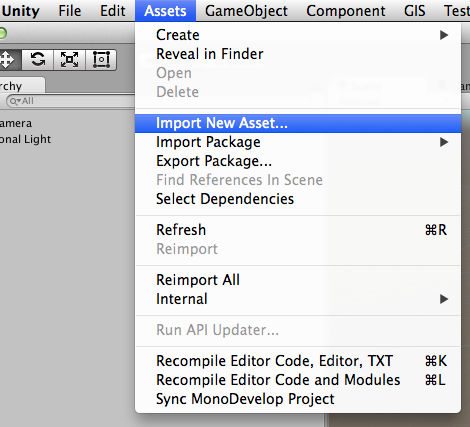
\includegraphics[width=200pt, height=200pt]{img/assetImport.png}
\bigskip

When the game is successfully loaded, you need to install the Myo Armband Manager. This is needed to allow Myo Armband gesture control with the game character. This is installed from the \href{https://support.getmyo.com/hc/en-us/articles/360018409792}{Myo Support Download Page.} Follow the Myo Installation guide until the Myo Armband can be used.

The final part of the setup is setting up the use of the microphone on the users machine. This is done be opening the Microphone Setup within Windows. Within this setting, go to 'Get Started'. From there, select which microphone you wish to use and follow the on-screen instructions.
\bigskip
\bigskip

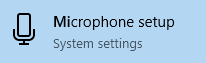
\includegraphics[height=65pt]{img/microphoneSetup.PNG}
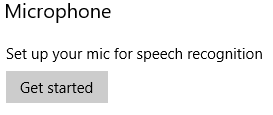
\includegraphics[]{img/micGetstarterd.PNG}
\bigskip

When the above steps are completed, the user can finally run and play the game. To do so, he/she needs to click the 'Play' within the Unity window.
\section{Research}

\includegraphics[width=\textwidth, height=150pt]{img/Research.jpg}
\bigskip

Before considering what gesture based project the development team wanted to create, a research phase was undertaken. Areas that were looked at included other gesture based projects, what hardware was available, and what sort of projects would work well with gesture based technology. After careful consideration, the team narrowed down a list of ideas and ultimately decided on creating a Unity game.

\bigskip

The team looked at viable options to incorporate gesture technology, with the Myo Armband being best suited for a Unity game. This was followed closely by what each technology could do to enhance the project. The team looked at certain types games that could be created using the technology that was decided upon. This swayed the development team to creating a 2D Platform style game.

\bigskip

Once the game has been decided and the hardware and software were chosen, the team looked at the "purpose of the application". This directed focus onto the design of the application, including the screens of the user interface and how it works by testing how pieces of
hardware/software could interact with each other, or be combined with gestures. The team also consider how gestures can be incorporated
into the application.

\bigskip

During the development of the project, a second research phase was completed. This research phase was conducted to discover possible solutions for navigating the Main Menu and Level Selection. The main gesture based technology that was studied was Speech Recognition. The team felt that Speech Recognition would add variety to the game, along with being extremely function-able.

\section{Original Project}

\includegraphics[width=\textwidth, height=180pt]{img/OriginalIdea.PNG}

\bigskip
The original plan for this project, was to create a 2D platform game, not too dissimilar to the original Super-Mario brothers game. The game character was to be completely controlled by the Myo armband.

The development team got quite deep into development with this project before things started going wrong. The project had gotten to a stage where the user could move the player left and right using the Myo armband, jump up and down using the armband, collect coins to score points, shoot bullets at an enemy, kill an enemy by jumping on it as well as jumping up against boxes to break them and get the coins sitting on top of them. The game also had a high score system implemented.
\bigskip

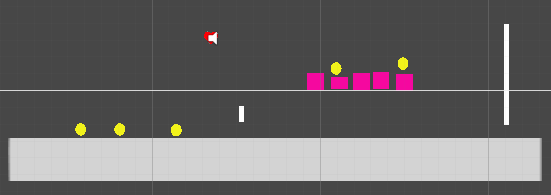
\includegraphics[width=\textwidth, height=150pt]{img/OriginalGame.PNG}

\bigskip

The movement that caused problems however was a rather trivial one. The development process ground to a halt when the team was trying to use Myo to get the player to jump onto an obstacle. This action would require the player to jump upwards, and then veer in the direction of the obstacle the user wanted the player to land on. This is extremely difficult to do with a Myo armband. The reason for this is that it would take two gestures in quick succession to pull this maneuver off. The user would have to do a jump gesture and a directional gesture one after the other. The armband, more often than not will try to read this as one unfamiliar gesture and will therefore not map it to an action. If the armband does read both gestures in succession, by the time the second gesture is acted upon, the player is already on the way back down and is therefore too late to make it onto the obstacle. 

\bigskip

The development team spent some time trying to come up with a work-around to this issue. The first idea they tried was to use momentum to carry the player onto an obstacle. This would entail having the player essentially run up and jump at the obstacle, relying on the build in physics of the unity engine to carry the player onto the obstacle. This method proved wildly inconsistent. Sometimes the player would just jump way over the obstacle, other times the player would just jump straight up in the air.

Another idea the development team tried, was to get the player to simply jump diagonally in the direction they were facing. This involved picking a point diagonally upwards from the current position of the player, and simply transforming the player to that point. While this was a little bit more accurate than the last approach, it was still completely unusable in a game scenario. Most of the time, the player would go along the X-axis before going up on the Y-axis, meaning the player would simply run into the obstacle before getting a chance to jump. Any times it did work, it looked extremely rough and twitchy. 

\bigskip

Eventually, a mutual agreement was reached between the team members to change the direction of the project. A lengthy brainstorming session took place, eventually giving birth to the idea of making an adaption of the Bubble Struggle game.


\section{Development Process}
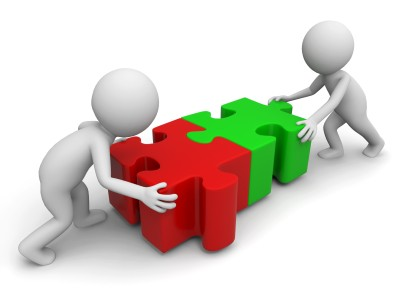
\includegraphics[width=\textwidth, height=180pt]{img/Development.jpg}

\bigskip

\subsubsection{Prototyping}
Once the development team decided to go with the Bubble Struggle adaption, they began developing a prototype level for the game that would be controlled using keys. This took some time because the logic of what happens to a bubble when it pops had to be worked out along with detecting all of the collisions. To use a more advanced collision detection system, the development team made use of the Unity Engine collision matrix. This collision matrix allows one so specify exactly what types of objects certain other objects can collide with. An collision matrix may look something like the following;
\bigskip

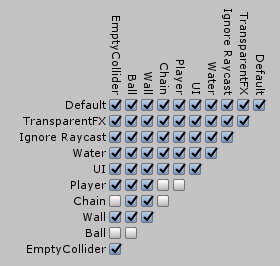
\includegraphics[width=150pt, height=150pt]{img/Matrix.PNG}

\bigskip

\subsubsection{Myo Integration}
Once the initial prototype was working with a mouse and keyboard, it was time to begin integrating the Myo gestures. How this integration works will be discussed in more detail in the next section. 

\subsubsection{Score System}
Once the development team had the player moving and shooting using the Myo controller, they began looking into some sort of a scoring system. The scoring system that was implemented works by starting a timer at the beginning of the level, and while displaying this timer to the user, decrement it by one every second. Once the game is over, i.e., if the player dies or clears all of the bubbles from the screen, the player's score is calculated by multiplying the time remaining on the timer by ten.

\subsubsection{High Score System}
With a scoring system up and running, it seemed logical to adds a high score system next. This high score system was easily implemented using Unity's "Player Prefs". This allowed the development team to use local storage to save the high score from each level in the game.

\subsubsection{Adding Levels}
Once the development team began working on adding levels to the game, a few issues arose. These issues will be discussed in more detail in the "Issues" section near the end of this document. The main objective of the development during this time was to make each level increase in difficulty. This was easily achieved by making the bubbles split into more children, increasing the speed the bubbles travel at as well as decreasing the game space making it harder for the player to dodge the bubbles. 

\subsubsection{Menu Creation}
With multiple levels made and a simple game prototype up and running, it was time to add in navigation capabilities. The development of this is discussed in more detail in the next section. It was at this point that the development team introduced speech recognition to the project. 
\clearpage

\subsubsection{Lives System}
As the development team were testing the application, they realized that it was incredibly difficult to pass any of the levels using the Myo gestures. This is due to some of the issues which were encountered, which will be discussed in more detail in the "Issues" section of the document. To give the user a more competitive gaming experience, the decision was made to add a lives system. The simple system works as follows;

\begin{itemize}
    \item Each level begins with three lives, as shown in the score board in the top left corner.
    
    \item Whenever the player gets hit by a bubble, they lose one life.
    
    \item If the number of lives left hits zero, the player dies and the game is over. 
    
    \item The player has one opportunity in each level to gain a life. This is achieved by shooting the heart that spawns at a random time in a random area in each level.
\end{itemize}

\subsubsection{Audio \& Sound Effects}

With a basic lives and scoring system in place, the development team now had a fully functioning game that could be completely controlled with gestures. However, the team felt that it was very dull and plain. The team wanted to create a more immersive experience for the user. The three pillars of immersive experiences are visual quality, sound quality, and intuitive interactions - \href{https://www.qualcomm.com/invention/cognitive-technologies/immersive-experiences}{Qualcomm}.

\bigskip

After reading through this website, the development team felt that they only had one of the three pillars needed to create an immersive experience for the user, intuitive interactions. In order to create such an experience, the development team new they needed to add audio and sound effects, as well as some visual displays. 

To achieve this, the development team added in a host of sound effects to the game. These sound effects include, making a "pop" sound when a bubble bursts, making a sound representing the shooting motion of the chain and hook, making the player say "ouch" to signify whenever he has been hit by a bubble, as well as adding a general back ground theme that plays throughout the entirety of run-time. 



\subsubsection{Art and Style}

\bigskip

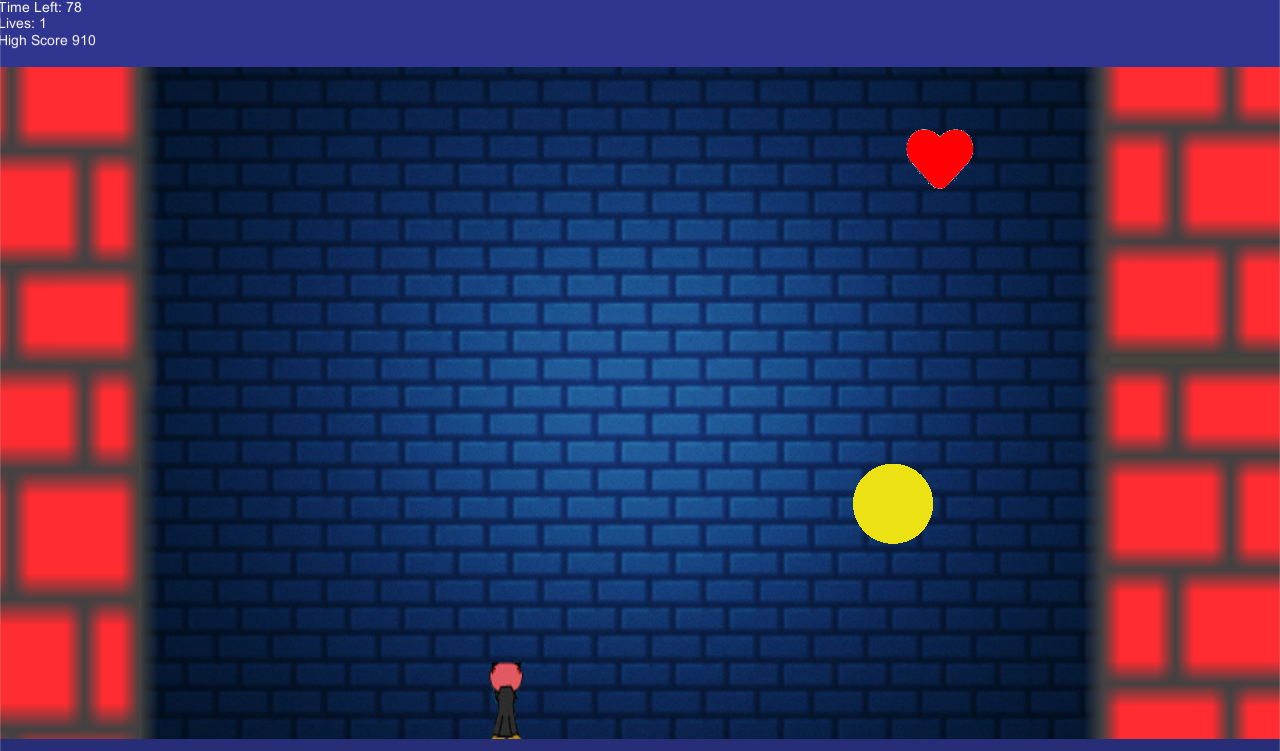
\includegraphics[width=\textwidth, height=180pt]{img/Art.PNG}

\bigskip

In order to make this game more aesthetically pleasing, the development team did a number of things. The first thing they did was create a visual representation of the player that wasn't just a white square. To do this, the team recreated the original game character using paint.net.

\bigskip

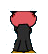
\includegraphics[width=200pt, height=100pt]{img/Player.png}

\bigskip

To add to this, the team also created a pixel art image of a brick wall, which serve as the boundaries to the game. The team also created a model for the chain and hook that looks quite like the chain and hook used in the original game. This image stretches upwards when is is shot, giving it the illusion of being thrown upwards towards the bubbles. There was also a back ground image of a blue brick wall.  


\section{Test Plan}


\subsection{Introduction}
This is the test plan that was implemented for the project in question.
\bigskip

This section covers in detail how the project was tested throughout development.
The goal at the end of this test plan's implementation, is to produce a project that has been rigorously tested to the extent that it should theoretically be fit for consumer use. 

\subsection{Test Items}
There is only one item to be tested in relation to this development.

\begin{itemize}
  \item Bubble Struggle.
\end{itemize}

\subsection{Features To Be Tested}

\begin{itemize}
  \item Player Movement.
  \item Bubble Bounce.
  \item Bubble Split.
  \item Shooting.
  \item High Score Calculation.
  \item Score Board.
  \item Menu System.
  \item Scene Graphics.
  \item Winning Conditions.
  \item Splash Screen.
  \item Background Music.
  \item Sound Effects.
  \item Voice Commands.
\end{itemize}

\subsection{Features Not To Be Tested}

\begin{itemize}
  \item Cross-Platform speech recognition - The speech recognition in this project needs access to the Windows Speech Recognition library in order to read in the speech gestures. This could not be tested on a non-Windows device.
\end{itemize}

\subsection{Approach}
The testing approach for this project was broken down into four sections.

\begin{itemize}
  \item Unit Test the features.
  \item Integration Test related features.
  \item System Test all features together.
  \item Acceptance Test entire project.
\end{itemize}

\subsubsection{Unit Test the Features}
This is performed on a very consistent basis throughout the development of the project. Each time one of the features listed above was completed, the development team would perform a unit test on that unit of the project to ensure it was working to their satisfaction before moving onto development of the next feature.

\subsubsection{Integration Test related features}
Integration testing was performed when the team had completed development of multiple related features in the project, and each feature had already passed unit testing. 
\bigskip

The development team would test how different features integrate with other completed features in the project. An example of this might be when the high score calculation feature is completed, as well as the scoreboard feature completed, the two feature could be integrated and test that they work together i.e., does the scoreboard automatically update when a new high score is calculated. 


\subsubsection{System Test on all features together}
The system testing took place towards the end of development because it required most of the game to be working and integrated in order to perform it. 
\bigskip

The system testing of this project involved testing how the game as a whole would react to certain conditions put on it. This involved testing the boundaries of the game i.e., does the game react in the correct way if the player just stands still until the game timer counts down to 0(The lives should get reset to 3 and the player should get redirected to the levels menu).

\subsubsection{Acceptance Test entire project}
The acceptance testing for this project will be done by the hypothetical customer (our peers) that the project is made for. This will be done when the project is fully completed and has passed all system testing.
\bigskip

The acceptance testing will be achieved by sending the customer the assets folder of the unity project so they can import the game into their own unity editor and play the game from start to finish themselves. They will then report back to the development the results of the acceptance tests.

\bigskip

All of the testing mentioned above will be done manually. The first three types of testing(Unit testing, integration testing, acceptance testing) will be white box testing whereas the acceptance testing will be black box testing i.e the customer does not know any details about how the game was made, they are just concerned with what it does.


\subsection{Item Pass/Fail Criteria}
The pass and fail criteria for this project differ depending on the particular feature that is being tested. These criteria are broken down into tables for a better visualization.

\subsection{Unit Tests}
\begin{center}
\begin{tabular}{ | m{5em} | m{4cm}| m{4cm} |  m{4cm} |} 
  \hline
  Feature & Test Case & Expected/Pass Result & Failed Result \\ 
  \hline
  Player Movement & Assert smooth movement & Moves left and right & Unsmooth movement / inability to move \\ 
  \hline
  Bubble Bounce & Assert bubbles bounce continuously & Bubbles bounce until they are popped & Bubbles do not bounce appropriately \\ 
  \hline
  Bubble Split & Assert bubbles split correctly & Bubbles split into 2 or more smaller bubbles & Bubbles do not split \\ 
  \hline
  Shooting & Player can shoot a chain & Chain continues until a collision & Chain does not shoot correctly or does not collide \\ 
  \hline
  Highscore & Assert that each score is calculated correctly & When new highscore is achieved, update local storage & Highscore is incorrectly calculated or not updated \\ 
  \hline
  Scoreboard & Assert scoreboard UI displays correctly & Scoreboard updates when player loses a life and the timer counts down & Scoreboard does not dynamically update or is not positioned correctly \\ 
  \hline
  Menu System & Assert menu system works smoothly & Smooth transition from each view depending on user interaction & Incorrect transition of views or no transition at all \\ 
  \hline
  Scene Graphics & Assert graphics correspond with game theme & The variation of graphics are accumulated to create a smooth view & Graphics not appearing or do not correspond with theme \\ 
  \hline
  Winning Conditions & Assert the player can complete a level & On completion of level by destroying all the bubbles, the levels menu is displayed & When the player completes a level, scene transition does not occur \\ 
  \hline
  Splash Screen & Assert the splash screen corresponds with game & The splash screen fades in for 3 seconds, remains for 3 seconds, and fades out for 3 seconds & Splash screen does not fade in or out, or does not auto-transition to main menu \\ 
  \hline
  Background Music & Assert background music works and fits with the game theme & The game music plays throughout the entirety of run time & The game music does not play throughout the entirety of run time \\ 
  \hline
  Sound Effects & Assert appropriate sound effects & The appropriate sound effect occurs when the corresponding event occurs & The appropriate sound effect does not occur when the corresponding event occurs \\ 
  \hline
\end{tabular}
\end{center}

\clearpage

\subsection{Integration Tests}
\begin{center}
\begin{tabular}{ | m{5em} | m{4cm}| m{4cm} |  m{4cm} |} 
      \hline
      Feature & Test Case & Expected/Pass Result & Failed Result \\ 
      \hline
      Player / Bubble Interaction & Assert that appropriate player and bubble interaction occurs & Bubble passes through the player and the lives decrease by one & Bubble does not pass through the player and the lives do not decrease by one \\ 
      \hline
      Score System & Assert scoreboard corresponds with highscore & Scoreboard updates automatically when a new highscore is achieved & Scoreboard does not update automatically when a new highscore is achieved \\ 
      \hline
      Game Routing & Assert the menu and game views interlace seamlessly & The user is routed to the correct game view depending on how they interact with a menu & The user is not routed to the correct view or routing is not working at all \\ 
      \hline
      Myo Gestures & Assert that Myo gestures perform appropriate player action & Player moves side to side and shoots with the corresponding gesture & Player does not move side to side and does not shoot with the corresponding gesture \\ 
      \hline
      Speech Recognition & Assert correct logistical action is performed & Correct logistical action is achieved with corresponding word or phrase & Correct logistical action is not achieved with corresponding word or phrase, or word or phrase is recognized and no action occurs \\ 
      \hline
      Audio Integration & Assert that the correct audio plays correspondingly & Audio plays correct sound effect louder than the background theme when the corresponding action occurs & Audio does not play (or not play at all) correct sound effect louder than the background theme when the corresponding action occurs \\ 
      \hline
\end{tabular}
\end{center}

\bigskip

\subsection{System Tests}
\begin{center}
\begin{tabular}{ | m{5em} | m{4cm}| m{4cm} |  m{4cm} |} 
      \hline
      Feature & Test Case & Expected/Pass Result & Failed Result \\ 
      \hline
      The Game and its Entirety & Assert that the full game can be played without bugs or glitches & The full game can be played over and over again without glitches or run-time errors, with all features working & There are previously unknown run-time errors in the game that prevents a smooth game-play \\ 
      \hline
\end{tabular}
\end{center}

\clearpage

\subsection{Acceptance Tests}
\begin{center}
\begin{tabular}{ | m{5em} | m{4cm}| m{4cm} |  m{4cm} |} 
      \hline
      Feature & Test Case & Expected/Pass Result & Failed Result \\ 
      \hline
      Bubble Struggle & Assert that game is complete from the point of view of the user & Users enjoy the game enough that it would be considered a finished product & The users advise changes that they seem to applicable to the game or has found previously unknown errors or glitches \\ 
      \hline
\end{tabular}
\end{center}

\bigskip

\section{Gesture Implementation}
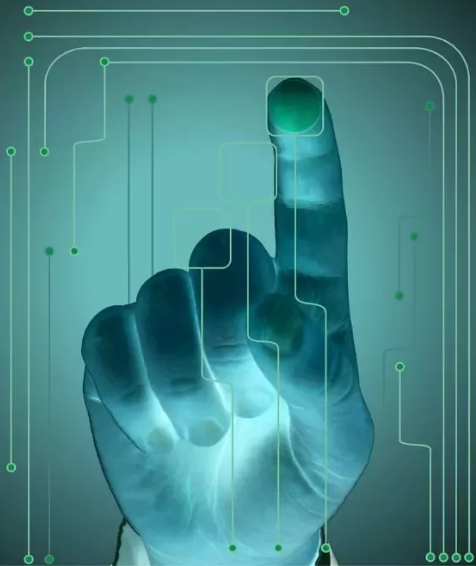
\includegraphics[width=\textwidth, height=180pt]{img/GestureImplementation.PNG}

\bigskip
The rational behind using the particular gestures that were implemented are discussed in a lot of detain in the "Gesture Considerations" document. This section is concerned with how these gestures were implemented and integrated into the project. This section is broken down into two sub-sections; Myo armband implementation, which will discuss how any gestures related to the Myo armband were implemented. The speech recognition and implementation will discuss how the speech recognition gestures were integrated to the project. For both sets of gestures, code snippets will be provided to help illustrate how these implementations work.

\subsection{Myo Armband Implementation}
There are three gestures that are read in from the Myo armband. 

\begin{itemize}
    \item Wave in.
    \item Wave out.
    \item Fist.
\end{itemize}

Before the development team could begin mapping actions to Myo gestures, they had to get a handle on the Thalmic hub. The thalmic hub also needs to be a singleton instance, so that the script can access it across multiple scenes. The script can get a handle on the Myo game object by using the following line of code:

\bigskip

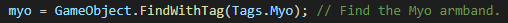
\includegraphics[width=\textwidth, height=30pt]{img/MyoGameObject.PNG}

\bigskip

This line of code searches the scene for a game object with a "myo" tag, and assigns that game object to the myo variable. Next, the script needs to use this Myo game object to access the thalmic Myo component on it. This is achieved by executing the following line of code:

\bigskip

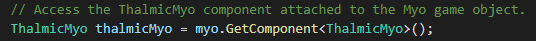
\includegraphics[width=\textwidth, height=30pt]{img/Thalmic.PNG}

\bigskip

Now that the script has a handle on the necessary component, the development team can begin mapping the gestures to actions.



\subsubsection{Wave In:}

The gesture to action mappings are quite easy to achieve. As discussed in the "Gesture Consideration" document, the wave-in pose should move the player to the left. This is achieved by constantly asking if the wave-in gesture is made inside of an update loop, and if it is, set the players movement to a negative number(negative along the x-axis) and multiply that number by the players speed.

\bigskip

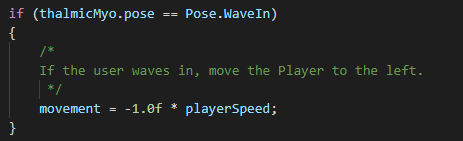
\includegraphics[width=\textwidth, height=100pt]{img/MoveLeft.PNG}

\bigskip

\subsubsection{Wave Out:}
As discussed in the "Gesture Consideration" document, the wave-out pose should move the player to the right.  This is achieved in the script by constantly asking if the wave-out gesture is made inside of an update loop, and if it is, set the players movement to a positive number(positive along the x-axis) and multiply that number by the players speed. 

\bigskip

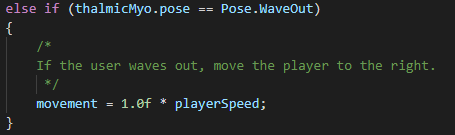
\includegraphics[width=\textwidth, height=100pt]{img/WaveOut.PNG}

\bigskip

\subsubsection{Fist:}

As discussed in the "Gesture Consideration" document, the fist gesture should shoot the hook and chain upwards at the bubbles. This is achieved in the script by constantly asking if the fist gesture is made inside of an update loop, if it is made, set a static variable from the "Chain" script to true. 

\bigskip

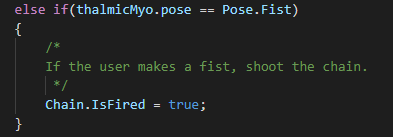
\includegraphics[width=\textwidth, height=100pt]{img/FistPose.PNG}

\bigskip

Once this static variable is set to true, the following code is triggered in the "Chain" script to shoot the chain into the air.

\bigskip

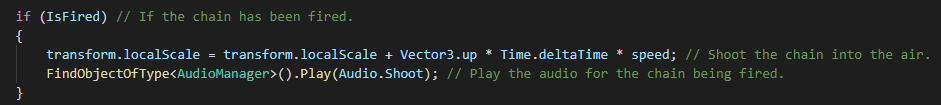
\includegraphics[width=\textwidth, height=80pt]{img/IsFired.PNG}

\bigskip



\subsection{Speech Recognition Implementation}
The speech recognition is implemented from the Unity Engine's keyword recognizer, which in turn, uses Windows microphone. Within the C\# script, this is done as follows:

\begin{enumerate}
    \item Import the Windows Speech library.
    \item Instantiate a new Dictionary object and Keyword Recognizer.
    \item Add recognized words to the dictionary, and map them to a function.
    \item Add the 'list' of the words within the dictionary to the Keyword Recognizer, along with the associated function.
    \item Add a 'listener' to recognize any spoken word within the dictionary/keyword recognizer.
\end{enumerate}
See screen-shot of code below for an example of how to implement.

\bigskip

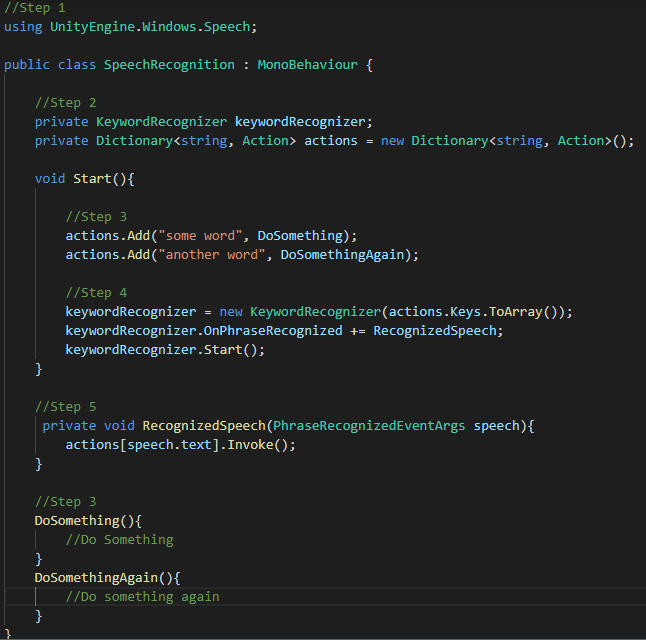
\includegraphics[width=\textwidth, height=\textwidth]{img/speechCode.PNG}

\bigskip

This snippet of code is found throughout the project and, as mentioned before, is used to navigate through the Main Menu, Levels Menu and In-Game Menu. Once 'keywordRecognizer.Start();' is called, it is constantly listening for a keyword to be spoken.

\section{Class Diagram}
This section is concerned with the data models and classes of the project. A UML sketch will be provided to better illustrate how this application is connected up and how the different elements behave. The entity relationships however, are not clearly shown in a UML for the fact that most of the scripts and classes in this project do not communicate with each other directly. The reason for this is because the scripts are attached to game objects and react only when certain game conditions are met.  The picture below provides a clearer picture of what is meant by this.

\bigskip

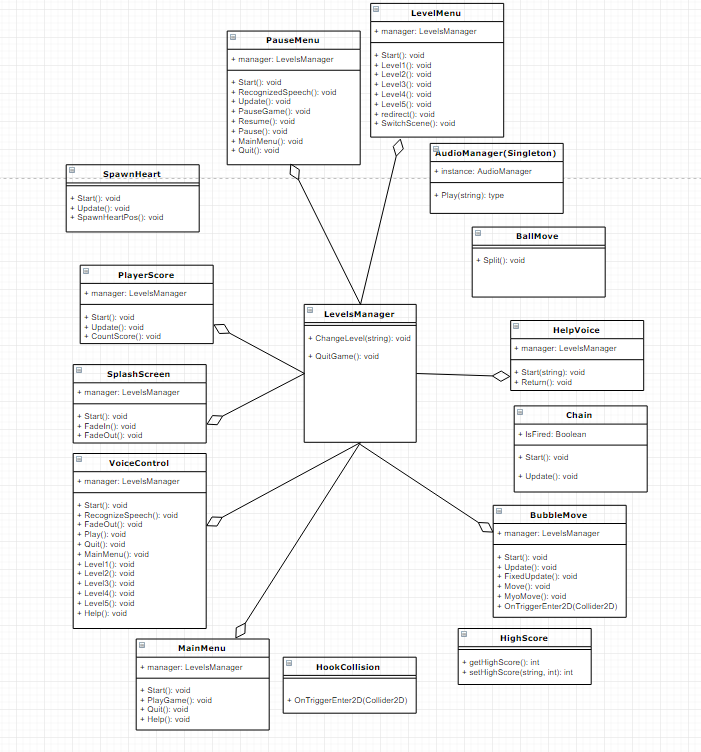
\includegraphics[width=\textwidth, height=\textwidth]{img/UML.PNG}

\bigskip

Here, it can be seen that a few classes have a direct relationship with the LevelsManager script. This is because these classes need to have the ability to dynamically change the scene of the game at run-time. Most of the classes here do not communicate directly in this game. However, most of them do communicate indirectly through in-game events. An example of this can be seen with the HookCollision and  the BallMove scripts. These scripts will only become related if the hook and chain collide with the bubbles at run-time. 



\section{System Architecture \& Distribution}
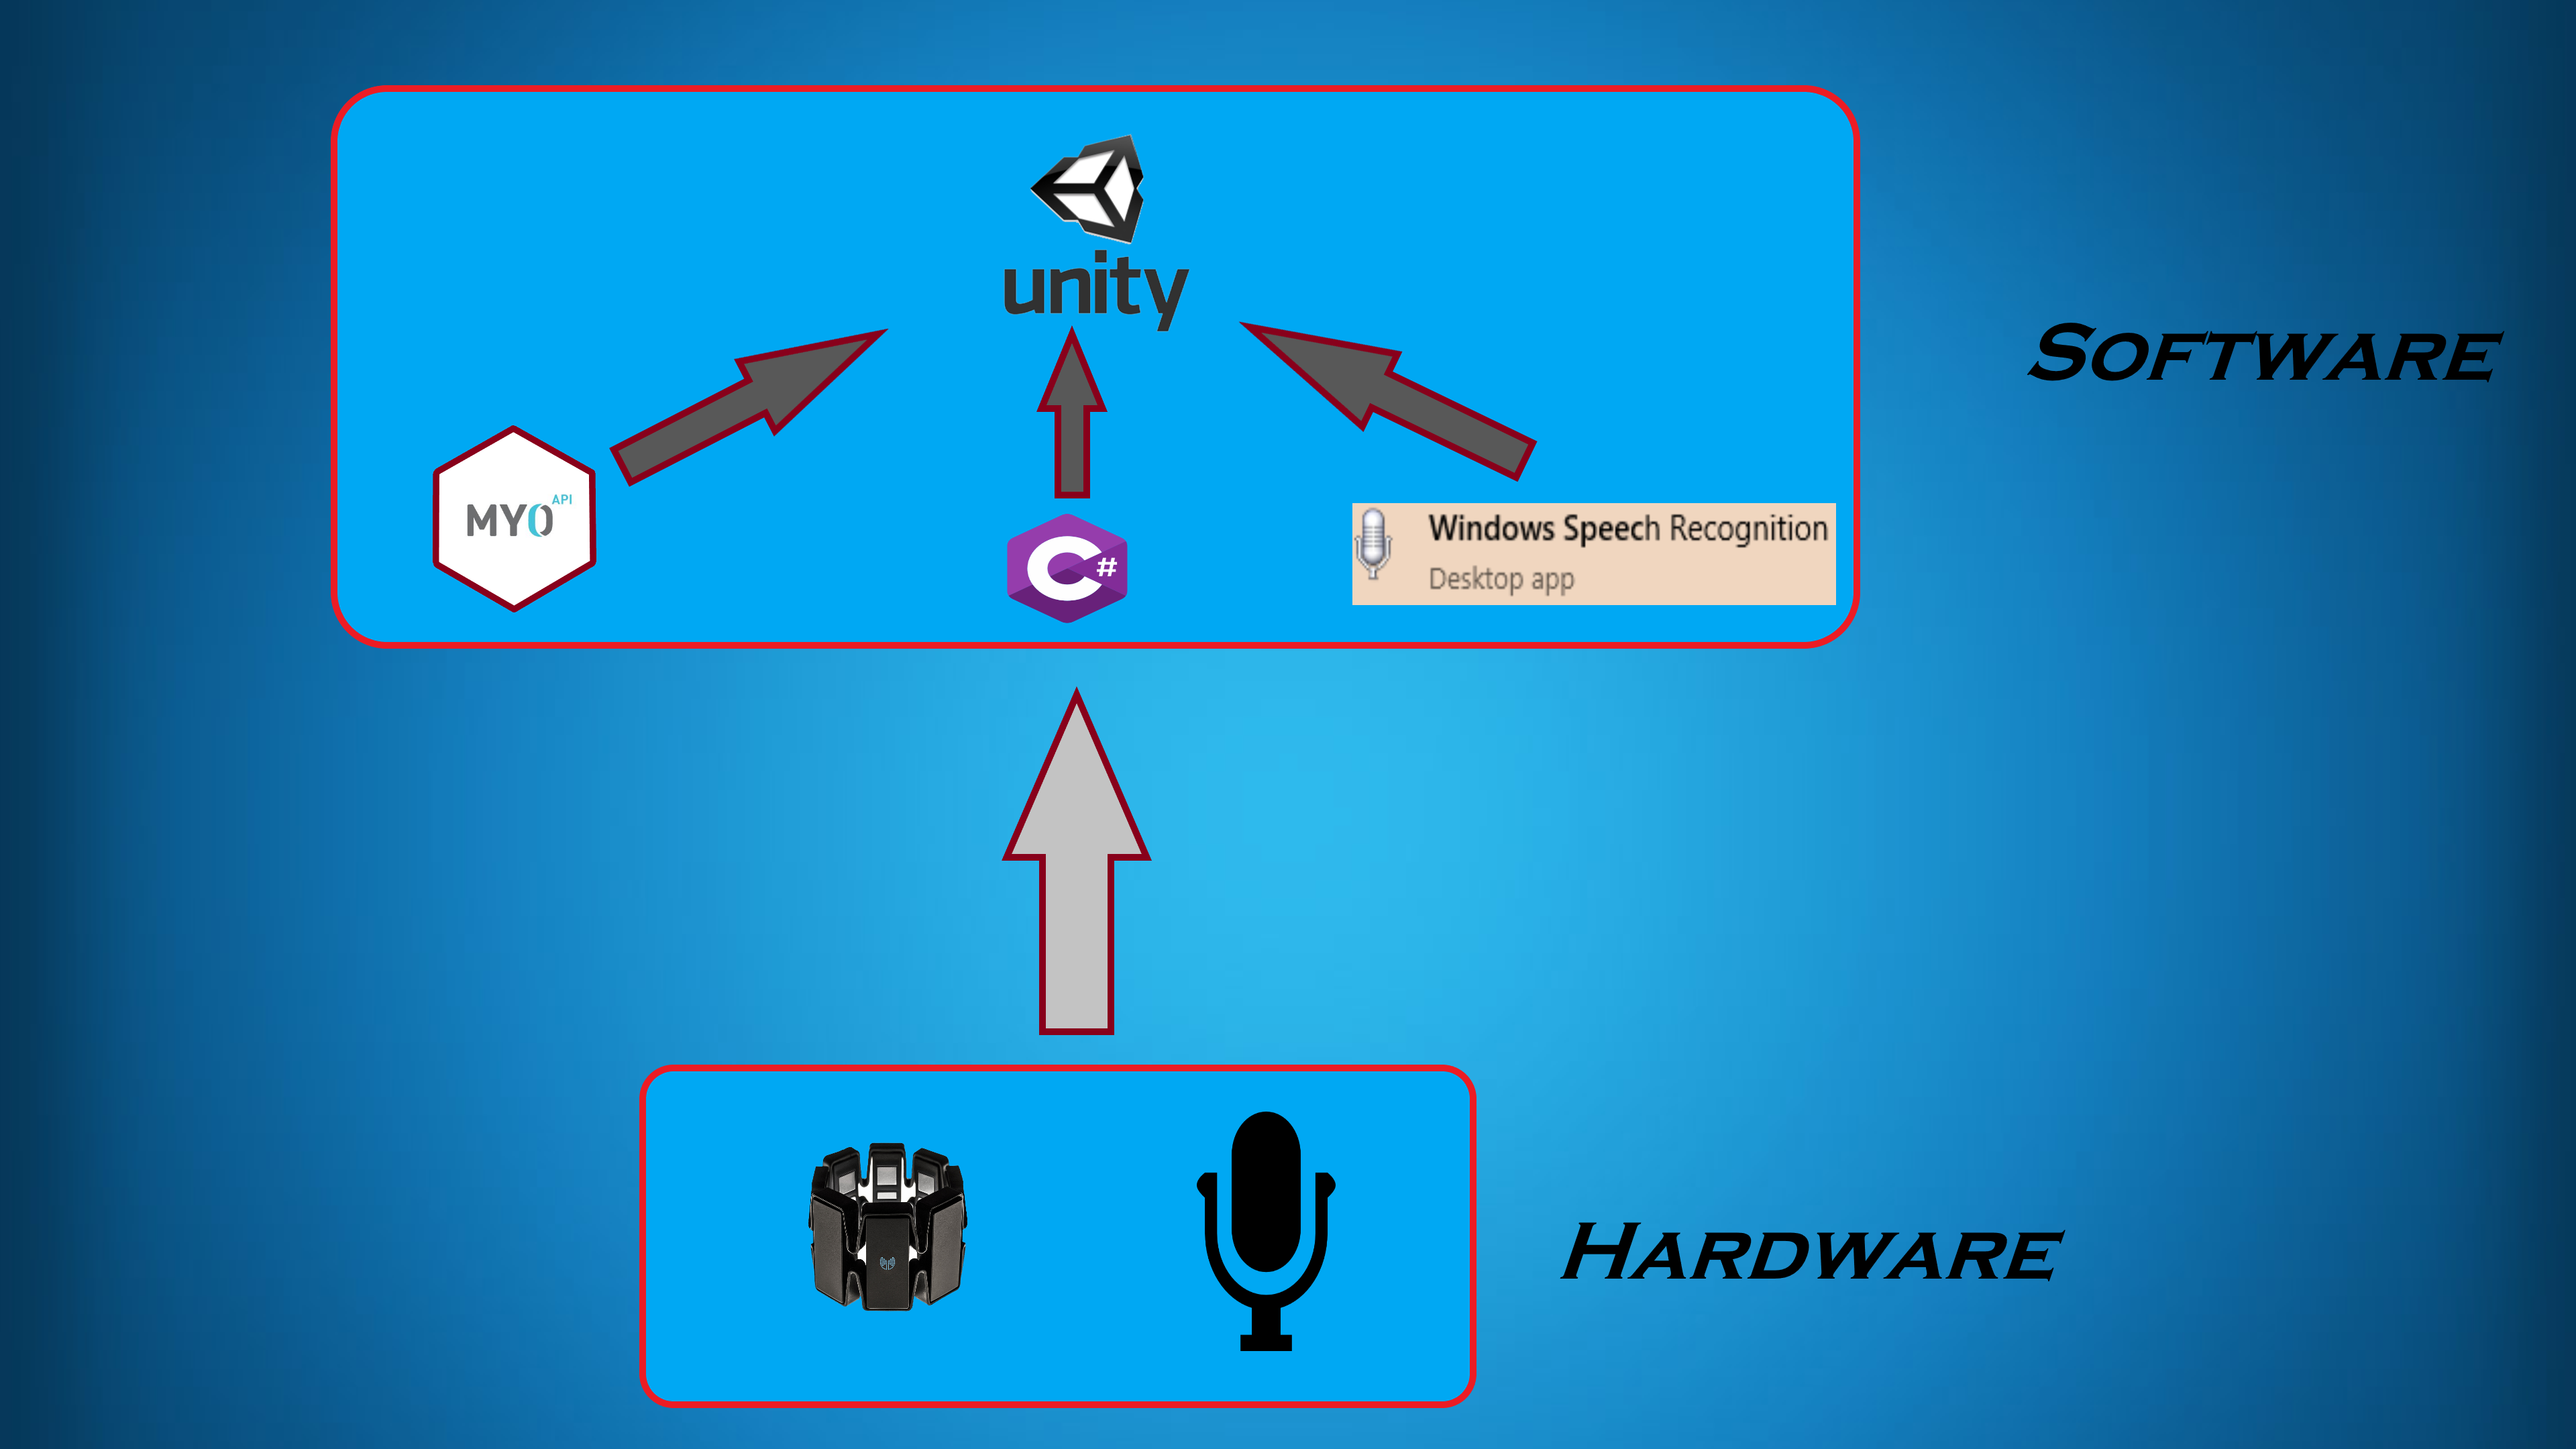
\includegraphics[width=\textwidth, height=150pt]{img/gestureProjectArchitecture.png}

\bigskip
The system architecture is a simplistic one for this project. This was intentional as it allowed for the development team to focus on the gesture based technology.

\bigskip

The hardware (microphone and Myo Armband) are external devices which are tied into the software. The Myo API is used to talk to the UnityEngine and allow it to be used within the game. The microphone uses windows speech recognizer to allow the Unity Engine to get a handle on the microphones input. This is all controlled within the C\# scripts. All of this allows for an even distribution of work load throughout the project.

\section{Hardware Justification}
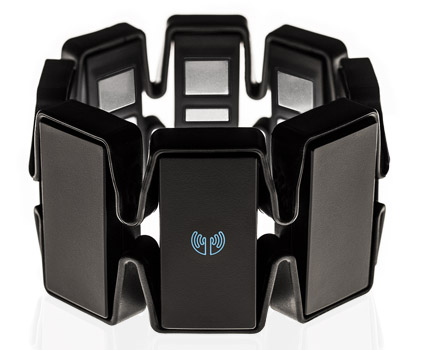
\includegraphics[width=\textwidth, height=180pt]{img/Hardware.jpg}

\bigskip

In this section, the reasons and rational for the hardware and technology used in this project will be discussed. 

\subsection{Myo Armband}
There were multiple technologies available to the development team for this project. Some of these technologies included;

\begin{itemize}
    \item Two Leap Motion Controllers.
    \item Two Kinect V2.
    \item Nine Myo Armbands.
    \item Two Hololens.
    \item Six Durovis Dive(Similar to Google Cardboard).
\end{itemize}

After much debate and consideration, the development team came to the conclusion that the Myo Armband would be the best suited technology for what the development team intended on making. 

\bigskip

The development team attended a few labs near the beginning of the semester in which the Myo armband was introduced and used. From the get-go, the development team liked the look and feel of the Myo armband and were curious to learn more. 

The Myo armband also made a lot of sense considering the fact that the team originally wanted to create a 2D platform game. Even though the original idea didn't work out, the transition in terms of the gestures used between the first game and the second, was not a huge one to make. 

Another, more trivial contributing factor was the fact that Myo armbands were in more abundance in the college. This made accessing the hardware required was never a huge issue. 

\bigskip

In hindsight, the development team feel that their decision to use the Myo armband was a wise one, and if they were given the same hardware options again, they would more than likely make the same decision.

\subsection{Speech Recognition}
The speech recognition was implemented late into the projects development. The development team wanted a 'hands-off' approach for navigating through the menu navigation. The main intention was to fully immerse the project fully into gesture based controls, with no keyboard input.

\bigskip

After discussing in length about how to achieve this, the development team decided on speech recognition. The Myo Armband was the initial solution for this issue, but this brought up a couple of issues. The first issue is that the development team wanted to include a variety of gesture based technologies. The second issue was that the Myo Armband was too inaccurate, along with being too slow to navigate through the games menus.

\section{Relevant Libraries}
The relevant libraries in this project include:

\begin{itemize}
    \item UnityEngine.Audio - This Unity library is necessary for allowing a script to play a piece of audio.
    \item UnityEngine.SceneManagement - This library is used to allow scenes to be switched dynamically at run-time from the sctipts.
    \item Thalmic.Myo.Pose - This library is used to allow a script to listen for gestures made from a Myo armband. It also allows the script to get a handle on what exact pose was made. 
    \item UnityEngine.Windows.Speech - This library allows the script to read in and recognise the speech that the application user speaks. This is necessary for any speech recognition. 
    \item UnityEngine.UI - This library allows the user interface to be dynamically edited at run-time through the C\# scripts.
\end{itemize}
\section{Game Walk-through}

When the game is initially loaded, the user is met with a splash screen which fades in and out. 

\bigskip
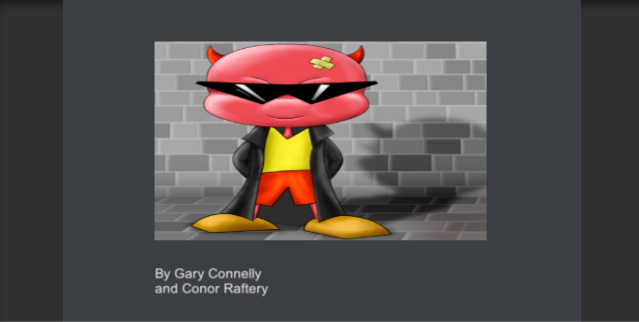
\includegraphics[width=350pt, height=180pt]{img/splashscreen.PNG}
\bigskip

This is followed by the Main Menu. This is controlled by speech recognition or the mouse. The user can quit the game from here, which will close the program. The user can also open up the help menu or levels menu from the main menu.

\bigskip
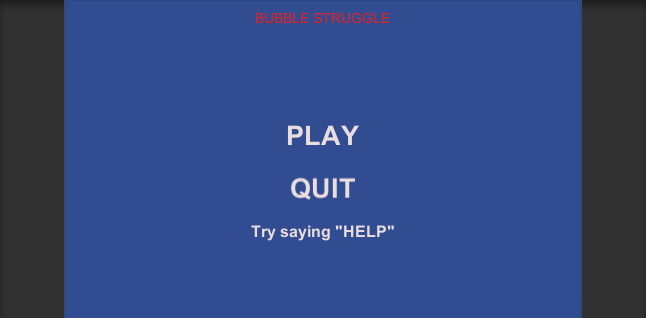
\includegraphics[width=350pt, height=180pt]{img/mainmenu.PNG}
\bigskip

When the help menu is opened, it displays text on how to use the game/program. This is very helpful for first time users. Within this menu, the user can navigate back to the main menu via speech recognition or a mouse click.

\bigskip
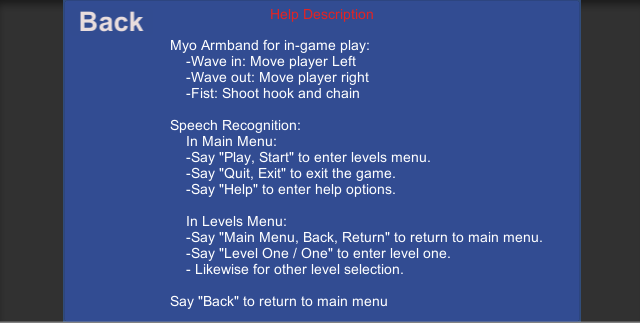
\includegraphics[width=350pt, height=180pt]{img/helpmenu.PNG}
\bigskip

When the levels menu is opened, it will display a list of all of the levels. The user can select any level they wish to play, with each level getting harder. The user can also navigate back to the main menu if they wish. This menu is also controlled my speech recognition or the mouse.

\bigskip
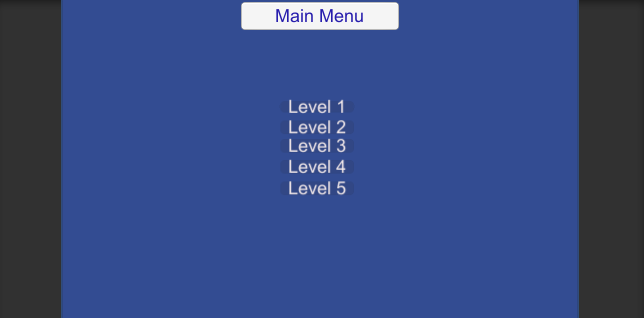
\includegraphics[width=350pt, height=180pt]{img/levelsmenu.PNG}
\bigskip

Once the user selects a level, they are met with the game screen. This is the main game of the project. The user controls the game character via the Myo Armband or by keyboard input. The user can either lose or win the game, in which case they will be returned to the levels menu.

\bigskip
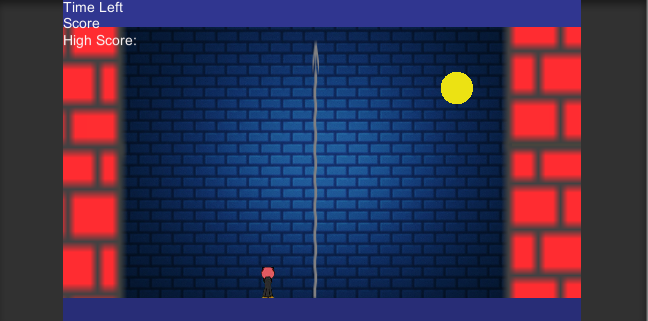
\includegraphics[width=350pt, height=180pt]{img/gamemenu.PNG}
\bigskip

The user may also pause the game via speech recognition, this will display a game view stating that the game is paused. The user can either resume the current game, or quit the current game and return to the main menu. This is done via speech recognition or by using the mouse.

\bigskip
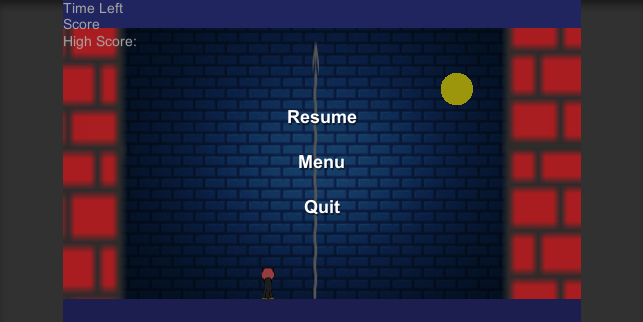
\includegraphics[width=350pt, height=180pt]{img/pausemenu.PNG}
\bigskip

\clearpage
\section{Issues}
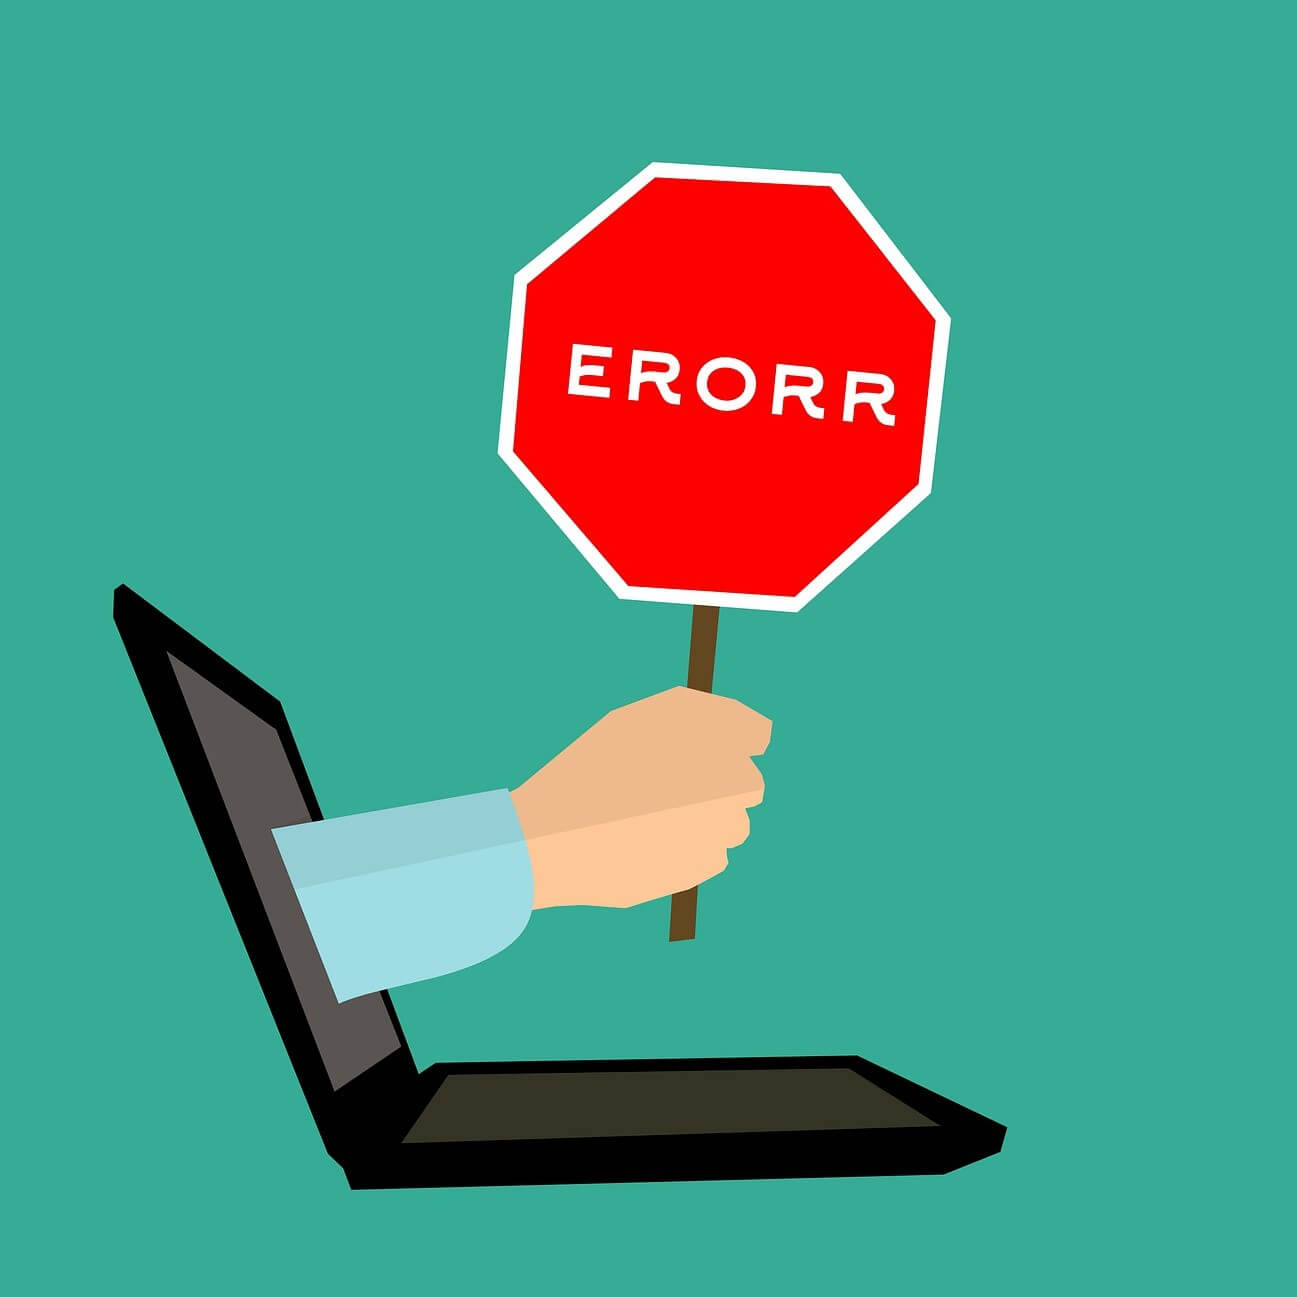
\includegraphics[width=\textwidth, height=180pt]{img/Error.jpg}

\bigskip
The development team came across multiple issues while developing this game. This section will discuss how these issues came about and how they were over come. The issues that will be discussed are as follows;

\begin{itemize}
    \item Myo Persistence.
    \item Myo Latency.
    \item Myo Accuracy. 
    \item Collisions.
\end{itemize}

\subsubsection{Myo Persistence}
The first real issue that the development team came across while developing the new project was persistence. The problem arose when the team tried to test the game across multiple levels in the one game play run-time. The Myo gestures just did not seem to be getting read in at all.

\bigskip

After much research and digging, the team realised the problem. The issue was that the way they had the script accessing the Myo was incorrect. Originally, the development team had a thalmic hub and Myo game object in every scene that needed it. Additionally, they were manually dragging and dropping the Myo game object into the script that needed to access it for every scene. This was incorrect. Because of the fact that the thalmic hub is a singleton, the instance that gets created in the first scene, automatically destroys the hub that tries to get created in the second scene. This process results in any script after the first scene having a null pointer where the team manually dragged and dropped the game object into it. 

\bigskip

The solution to this problem was to create only once thalmic hub and Myo game object in the very first scene. This hub would automatically persist across multiple scenes. The correct way for the script to gain access to the Myo was by following the steps outlined in the "Gesture Implementation" section.

\subsubsection{Myo Latency}

Another issue that the team ran into was latency. Depending on the device that the user was using, for example a slow laptop, the reaction time between the moment the gesture was made to when the action was executed, was slightly delayed. This was a huge disadvantage to the user in a game where quick reactions is the difference between winning and losing. The get around this issue, the development team had to consider ways to make the game more fair for the user in cases like this. The solution they came up with was to integrate a three lives system.

\subsubsection{Myo Accuracy}

Sometimes the gestures the user makes would map to a different action to the one intended. An example of this might be when the player is waving in to move the player left, and the Myo reads it as a fist and shoots the chain instead of moving. 

\bigskip

The source of this issue is mostly due to the nature of the game. In the latter levels, the user might be in the situation where there are a lot of bubbles bouncing around the screen that the user is trying to avoid. When this happens, the natural instinct for the user is to tense up their arm. This tension could cause inaccurate reading coming from the Myo, for example reading a fist gesture when it is really a wave-in gesture. 
The solution to help mask the consequences of this issue was also to integrate a three lives system to the game.

\subsubsection{Collisions}

When the development team decided to integrate the three lives system, a few more issues followed. Before this system was added, the player only needed to get hit once by a bubble and the game would be over. Because of this, the development team did not need to worry about the physics that played out between the player and bubble once they collided. Once the lives system was implemented, if a bubble hit the player at a weird angle, the player would lose a life but the bubble might trickle along the ground and stop bouncing. This was obviously a big issue because the player can only shoot upwards and night sideways, meaning the level cannot be completed.

\bigskip

The first thing the development team did to help solve this issue, was make the collider on the player a trigger. This way, the collision would still trigger between the bubbles and the player, but would not act out the physics of the collision. The bubbles would appear to pass through the player. However, with this change, the player would not collide with anything, including the boundary walls. To fix this issue, the team had to create an empty game object and make it a child element of the player. They then had to put a box collider on this empty object. The then had to, using the collision matrix(discussed in the "Development Process" section) allow that collider to only collide with the boundaries.

\bigskip

With these changes implemented, the player could now hit against the walls, while allowing the bubbles to pass through him, still triggering the collision. 

\section{Learning Outcomes \& Conclusion}
Although the development team were quite happy with the outcome of this project, there are certain aspects that would be reconsidered. If this project was to be redone, more time would be put into considering the inclusion of a multitude of gesture based hardware. For example, the use of image recognition technology.

\bigskip

The development team feel they should have foreseen the issues of the original project, in particular the issues that have previously been mentioned within this document (Making the game character move and jump simultaneously). Had they foreseen these issues, they would have had more time to work on additional technologies. The team have refined a magnitude of skill, such as version control, proper planning and working with new and innovative technologies, during the development of this project.

\bigskip

Given more time, the development team would have liked to add animation to the characters movements, but they are overall happy with the finished product.

\end{document}
